\documentclass{article}

\usepackage{framed}
\usepackage{hyperref}
\usepackage{verbatim}
\usepackage{graphicx}
\usepackage{amsmath}

\addtolength{\textwidth}{1in}
\addtolength{\textheight}{1in}
\addtolength{\hoffset}{-0.5in}
\addtolength{\voffset}{-0.5in}


\renewcommand{\familydefault}{\sfdefault}
\usepackage{helvet}


\newcommand{\LocARNA}{\textsc{LocARNA}}
\newcommand{\LocARNAP}{\textsc{LocARNA-P}}
\newenvironment{ttbox}{%
  \begin{framed}\begin{minipage}{1.0\textwidth}\tt}%
{\end{minipage}\end{framed}\noindent}


\title{\LocARNAP{} Manual:\\ Computing Match Probabilities and
  Reliabilities in \LocARNA{}'s Probabilistic Mode} 

\author{Sebastian Will\\[6pt]
\normalsize
  \emph{Computer Science, University Freiburg, Freiburg, Germany}\\
\normalsize
  \emph{CSAIL, MIT, Cambridge, MA, USA}
} 

\date{\LocARNA{} version 1.6}

\begin{document}

\maketitle

\section*{Overview}

This document is part of the documentation of the tool package
\LocARNA{}. The package \LocARNA{} consists of several tools for the
comparative analysis of RNA based on simultaneous alignment and
folding (SA\&F)~\cite{sankoff85}. This document describes the features
of \LocARNAP{}~\cite{Will:LocARNAP:unpublished}, i.e. the part of the package that
extends the original functionality of \LocARNA{}~\cite{Will:etal:_infer_non_codin_rna_famil:PLOS2007} by
features based on the efficient computation of match
probabilities. These features comprise
\begin{itemize}
\item Multiple alignment based on probabilistic consistency
  transformation
\item Assessment of local alignment quality by reliability profiles
\item Locating RNA motifs in reliability profiles
\item De-novo prediction of structural, non-coding RNA
\item Calculating pairwise partition functions and sequence and
  structure match probabilities
\item Refining genome-wide screens for putative non-coding RNA
\end{itemize}

We describe the installation of the \LocARNA{} package and the usage
of the \LocARNAP{} functionality. Finally, we provide detailed
instructions and script for refining genomic screens for the de-novo
prediction of structural RNA with \LocARNAP{}.

\section{Installation}

The package \LocARNA{} is distributed as source code under license
GPLv2 and available for download at
\begin{center}
  \url{http://www.bioinf.uni-freiburg.de/Software/LocARNA/}.
\end{center}
%
We provide installation instructions for a recent GNU/Linux-based
desktop operating system like Ubuntu or Fedora. 

All but the very low-level functionality of \LocARNA{} requires a recent
installation of the Vienna RNA package. If the package is not
available on your system, please download from
\begin{center}
  \url{http://www.tbi.univie.ac.at/~ivo/RNA/}
\end{center}
and install this package
following its installation instructions.

To install \LocARNA{} on your system, download the latest release from
\begin{center}
  \url{http://www.bioinf.uni-freiburg.de/Software/LocARNA/}.
\end{center}
At this time the latest release is Version 1.6 and directly obtained
from
\begin{center}
  \url{http://www.bioinf.uni-freiburg.de/Software/LocARNA/Releases/locarna-1.6.tar.gz}.
\end{center}

\LocARNA{} is installed from the command line by running the commands

\begin{ttbox}
  tar xzf locarna-1.6.tar.gz\\
  cd locarna-1.6\\
  \\
  ./configure \\
  make\\
  make install\\
\end{ttbox}
These commands will compile the package and install it under directory
\texttt{/usr/local}. 

\paragraph{Non-standard installation} For installing \LocARNA{} in a
different directory hierarchy or when the Vienna programs are not in
the default search path, one controls this by options of
\texttt{configure}. \texttt{configure --help} provides a complete list
of configuration options. Most importantly, the
installation path is controlled by
\begin{ttbox}
  ./configure --prefix=LOCARNA\_INSTALLATION\_PATH
\end{ttbox}
 
The installation path of the Vienna RNA package is controlled by
LocARNA-specific options and environment variables for
\texttt{configure}.%
The \texttt{configure} option 
\begin{ttbox}
  --with-vrna=VRNAPREFIX
\end{ttbox}
selects the installation directory of the Vienna RNA library to
\texttt{VRNAPREFIX}.
%
Specific names and paths of executables are controlled by environment
variables:
\begin{description}
\item[RNAfold] name of executable RNAfold (def=RNAfold)
\item[RNAplfold] name of executable RNAplfold (def=RNAplfold)
\item[RNAalifold] name of executable RNAalifold (def=RNAalifold)
\item[TCOFFEE] name of executable tcoffee (def=t\_coffee)
\end{description}

Note that T-Coffee is not used in probabilistic mode and therefore
need not be installed for the functions described in this
document. However, for using the tool
\texttt{locarnate}~\cite{Otto:Will:Backofen:_struc_local_multip_align_of_rna:CGB08}
of the package, T-Coffee is required. It is available from
\url{http://www.tcoffee.org/Projects_home_page/t_coffee_home_page.html}.

For aligning large sequences it is advised to use the option
\begin{ttbox}
  --enable-large-pf
\end{ttbox}
when calling \texttt{configure}. This option avoids under- and
overflows when computing the partition function by activating high
precision floating point arithmetic.

\section{Quick Start}

This section describes standard functionality and usage by a small
example. The distribution contains some example input in the
subdirectory \texttt{Examples}. In general \LocARNA{} is controlled
from the command line. We assume that \texttt{Examples} is the current
directory.

We are going to align the sequences specified in the file archaea.fa:
\begin{framed}
  \verbatiminput{example.fa} 
\end{framed}

These sequences are multiply aligned by running
\begin{ttbox}
  mlocarna --probabilistic --consistency-transformation archaea.fa
\end{ttbox}
Due to the options \texttt{--probabilistic
  --consistency-transformation} the alignment is based on match
probabilities and probabilistic consistency transformation, which increases the accuracy over the default operation of \texttt{mlocarna}.

The command writes the following text output to standard out.
\begin{framed}
  \verbatiminput{example.output}
\end{framed}

After some progress messages, the output contains the generated
alignment, the \texttt{RNAalifold} consensus structure for the
generated alignment, and reliability information.  The call will
furthermore generate a directory \texttt{archaea.out} containing
result and input files.


\section{Central Functionality: Computing Multiple Alignments and
  Match Probabilities}

This section details the probabilistic mode of the multiple alignment
tool \texttt{mlocarna}, which is activated by the option
\texttt{--probabilistic}.
%
In this mode, \texttt{mlocarna} will compute pairwise match
probabilities for all pairs of your input sequences. It computes base
match \emph{and} base pair match probabilities. These probabilities
are technically defined as probabilities of a respective sequence or
structure match in the Boltzmann ensemble of alignment/consensus
structure pairs~\cite{Will:LocARNAP:unpublished}.

For fast reference, the tool \texttt{mlocarna} provides an overview of
its various options by
\begin{ttbox}
  mlocarna --man
\end{ttbox}

In general, \texttt{mlocarna INPUT.fa} accepts a fasta file INPUT.fa
and writes text output to standard out and writes result files,
intermediary files and input files to a target directory. This output
directory defaults to \texttt{INPUT.out} and can be specified by
\texttt{mlocarna --tgtdir DIR}.

The call
\begin{ttbox}
  mlocarna --probabilistic --consistency-transformation --tgtdir TGT IN.fa 
\end{ttbox}
results in the following actions and output.

\begin{itemize}
\item read the \emph{input sequences} and their names from IN.fa
\item compute base pair probabilities for all input sequences (runs
  \texttt{RNAfold -p}). Write sequences and base pair probabilities to
  files in subdirectory TGT/input using proprietary pp-format
\item compute partition functions and (sequence and structure) match
  probabilities for all pairs of input sequences. Write match
  probabilities to files in \texttt{TGT/probs/bmprobs} (base match)
  and \texttt{TGT/probs/amprobs} (arc match). In this step
  \texttt{mlocarna} calls the tool \texttt{locarna\_p}.
\item consistency transform sequence and structure match
  probabilities. Write transformed probabilities to files in
  \texttt{TGT/probs/bmprobs-cbt} and \texttt{TGT/probs/amprobs-cbt}
\item Compute all pairwise alignments and generate guide tree (by the
  pair group method algorithm). Write the guide tree to
  \texttt{TGT/results/result.tree}.
\item Perform progressive alignment for constructing the multiple
  alignment.  In each progressive alignment step \texttt{mlocarna}
  calls the low-level tool \texttt{locarna} in order to perform a
  maximum expected accuracy alignment based on the computed (and
  transformed) match probabilities. In each progressive step, write
  the resulting intermediary alignments to \texttt{TGT/intermediates}
  and the final alignment to \texttt{TGT/results/results.aln}.
\item run \texttt{RNAalifold -r} on the final alignment and write
  output to standard output and the directory \texttt{TGT/results}.
\item Compute a reliability profile and a reliability dot plot
  (containing reliabilities of each base pair in the consensus
  structure). Experimentally, compute reliabilities projected to each
  input sequence and predict MEA structures for each sequence.  Write
  the results to to standard out and \texttt{TGT/results}.
\end{itemize}
%
We list some important options that modify \texttt{mlocarna}'s behavior.
\begin{itemize}
\item The actions of \texttt{mlocarna} are reported verbosely when
  using option \texttt{-v} and even more verbose with option
  \texttt{--moreverbose}.
\item Omitting the option \texttt{--consistency-transformation} skips the
consistency computation and runs the progressive multiple alignment on
the untransformed match probabilities.
\item \texttt{--max-diff=$\Delta$} controls a heuristic in
  \texttt{mlocarna} that trades computation time vs. alignment
  accuracy. It restricts the difference $|k-(m/n)i|$ for alignment
  cuts $(i,k)$, where $n$ and $m$ are the sequence lengths.  This
  will, in particular, disallow matches of positions $i$ and $k$ where
  the above difference is larger than $\Delta$. This restriction is
  applied to all alignment and match probability
  computations. $\Delta=60$ appeared to be a conservative restriction
  in the Bralibase benchmark.
\item \texttt{--plfold-span=$L$} and \texttt{--plfold-winsize=$W$}
  restrict the base pair size when computing base pair probabilities
  by calling \texttt{RNAplfold} with span $L$ and window size $W$
  (default $W=2L$).
\item \texttt{--mea-beta=$\beta$} Weight of base pair match
  contribution in probabilistic mode. (Default $\beta=200$,
  however $\beta=400$ yields better results in Bralibase benchmark.)
\item \texttt{--threads=$k$}. Use $k$ threads for distributable
  computations in mlocarna. With this option \texttt{mlocarna} gains
  significant speed on multi-cores.
\item \texttt{--iterate} or \texttt{--iterations=$I$} Perform
  iterative refinement for respectively $1$ or at most $I$ iterations
  after the progressive alignment.
\end{itemize}

For aligning up to about 15 sequences of lengths up to a few hundred nt (like most
RNAs in Rfam and as tested in the Bralibase benchmark), a recommended parametrization is e.g.
\begin{ttbox}
  mlocarna --probabilistic --consistency-transformation --iterations=2 $\backslash$ \\
  \hphantom{mlocarna} --max-diff=60 --mea-beta=400 % $\backslash$ \\
  % \hphantom{mlocarna} 
  --tgtdir TGT IN.fa
\end{ttbox}

For aligning very long sequences, e.g. 10 sequences of length of a few
thousand nt, we recommend the use of \texttt{--plfold-span} and
multiple cores, e.g.
\begin{ttbox}
  mlocarna --probabilistic --consistency-transformation --iterate -v $\backslash$ \\
  \hphantom{mlocarna}  --max-diff=100 --mea-beta=400 --threads=8 --plfold-span=120 $\backslash$ \\
  \hphantom{mlocarna} --tgtdir TGT IN.fa
\end{ttbox}

\section{Reliability Profiles}

A reliability profile of \LocARNAP{} consists of a sequence and a
structure reliability for each alignment column. The weighted sum of
both \emph{column reliabilities} is called \emph{total column
  reliability}.  Working with \LocARNAP's reliability profiles of
alignments always starts by creating a multiple alignment of the
alignment sequences using \texttt{mlocarna --probabilistic} as
discussed in the previous section. The sequences are given to
\texttt{mlocarna} as input in fasta format.

\subsection{Plotting Reliability Profiles}

We provide a tool \texttt{reliability-profile.pl} that generates
reliability profile plots as show in Figure~\ref{fig:relprof}. Note
that the use of this script requires a working installation of the
statistics package \texttt{R}. A text-based version of such a profile
is already given in the text output of \LocARNAP{}.

\begin{figure}[h]
  \centering
  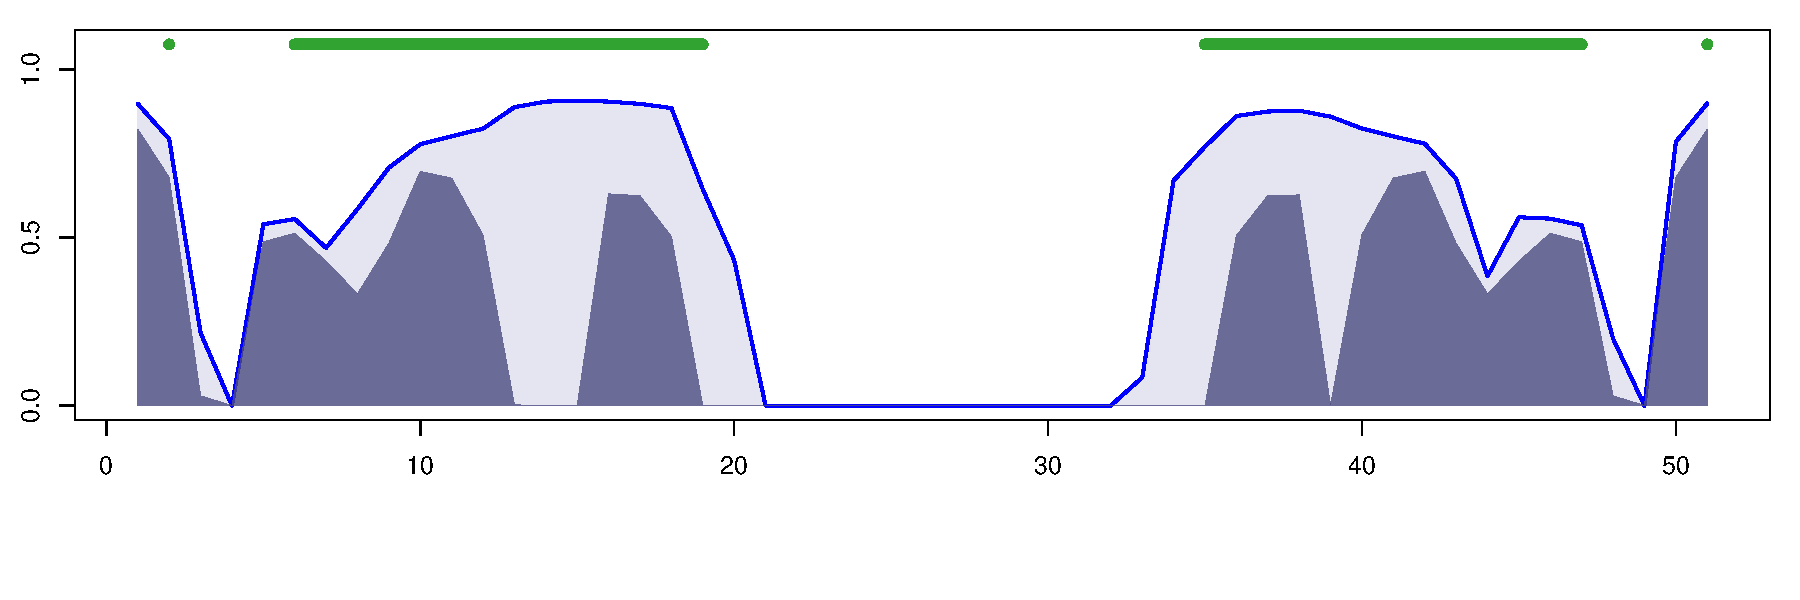
\includegraphics[width=0.6\textwidth]{Figs/relprof.pdf}
  \caption{Reliability profile plot of the small example
    \texttt{example.fa} as generated by
    \texttt{reliability-profile.pl}}
  \label{fig:relprof}
\end{figure}

A complete overview of the options of the tool is obtained by
\begin{ttbox}
  reliability-profile.pl --man
\end{ttbox}

For generating the plot of Figure~\ref{fig:relprof}, one runs
\begin{ttbox}
  mlocarna --probabilistic --consistency-transformation archaea.fa
\end{ttbox}
as in the Quick Start section followed by
\begin{ttbox}
  reliability-profile.pl archaea.out
\end{ttbox}
This generates the plot and writes it to the file \texttt{rel.pdf} in
pdf format. Note that the script requires the target directory
\texttt{archaea.fa} of the above \texttt{mlocarna} run as
input. Recall that \texttt{mlocarna} computes and stores the profile
data in the target directory.

In its default setting, the script \texttt{reliability-profile.pl}
predicts the regions of highest reliability and marks them by green
lines in the plot. Details of this prediction and how to control it
are described in the next section. The prediction can be turned off by
the option \texttt{--dont-predict}.

The following options of \texttt{reliability-profile.pl} control its
output for pure profile plotting (without controlling the prediction). 

\begin{description}
       \item[\texttt{--seqname=seqname}]       Project to sequence name
       \item[\texttt{--dont-predict}]          Turn off predicting. (defaults to on)
       \item[\texttt{--title=title}]           Title of plot
       \item[\texttt{--out=filename}]          Output filename
       \item[\texttt{--offset=pos}]            Offset of sequence in genome
       \item[\texttt{--signals=list}] List of (from,to,orientation)
         triples to specify signals that will be shown in the plot.
         One provides the list as string "from0 to0 orientation0;from1
         to1 orientation1 ...". Its possible to specify multi-range
         signals by from0a to0a from0b to0b ...
       \item[\texttt{--structure-weight=w}]    Weight of structure against sequence (1.0)
       \item[\texttt{--show-sw}]               Show the influence of structure weight in the plot
       \item[\texttt{--dont-plot}]             Skip plotting, only output prediction
       \item[\texttt{--write-R-script}]        Write the R script
       \item[\texttt{--revcompl}]              Plot (and fit) the reverse complement
       \item[\texttt{--output-format=f}]       Output format (f = pdf or png, defaults to pdf)
       \item[\texttt{--show-fitonoff}]         Show the on/off values for the fit

\end{description}

\subsection{Reliability Profiles for Locating RNA Motifs}

Likely locations of RNA motifs can be predicted from the reliability
profile using the script \texttt{reliability-profile.pl}, which will
also show the prediction in the resulting plot.  Note that the script
delegates the actual prediction to the low-level tool \texttt{fit},
which never has to be called directly by most users.

The prediction of RNA motifs can be controlled in various ways due to
the following options of \texttt{reliability-profile.pl}.

\begin{description}
       \item[\texttt{--fit-penalty=$\delta$}]  Penalty for on/off switching in fit
       \item[\texttt{--fit-once-on}]           Restrict fitting to being exactly once on
       \item[\texttt{--structure-weight=$sw$}] Weight of structure
         against sequence (1.0)
       \item[\texttt{--beta=$\beta$}]          Inverse temperature beta
       \item[\texttt{--revcompl}]              Plot and fit a reverse complement
       \item[\texttt{--write-subseq}]          Write the subsequence of fit
\end{description}

The parameters $delta$, $sw$, and $\beta$ control the actual
predicting procedure that fits a two-step-function to the signal of
total column reliability. $\delta$ is a penalty for switching between
on and off in the two-step-function. $sw$ is a factor that weights
structure reliability against sequence reliability. Large $sw$ result
in strong emphasis of the structure signal for the prediction. In
practice, it can be useful to set $sw=2$ or $sw=3$. $\beta$ controls
the optimization procedure for estimating optimal on and off values
for the two-step-function. \texttt{--fit-once-on} increases the
accuracy, when predicting boundaries of a single RNA motif in an
alignment by using this prior knowledge. \texttt{--revcompl} will plot
the profile of the reverse complement of the alignment and also
predict the RNA motif region(s) for the reverse complement.


\subsection{Evaluation of Existing Alignments by Reliabilities and
  Reliability Profiles for De-novo Prediction}

\LocARNAP{} allows the evaluation of existing alignments due to the
\LocARNA{} alignment model. In particular, this yields reliability
scores that discriminates true non-coding RNA regions from other
regions with high accuracy. This can be used in refining genome-wide
de-novo prediction of non-coding RNA.

Assume, an existing alignment in file \texttt{input.aln}. We further
need the unaligned sequences of \texttt{input.aln} in a file
\texttt{input.fa}.  For evaluating the alignment in
\texttt{input.aln}, one first calls \texttt{mlocarna} on the sequences
in \texttt{input.fa}, like
\begin{ttbox}
  mlocarna --probabilistic input.fa --tgtdir TGT
\end{ttbox}
The alignment of \texttt{input.aln} is now evaluated by
\begin{ttbox}
  mlocarna --evaluate input.aln input.fa --tgtdir TGT
\end{ttbox}
The option \emph{--tgtdir} can be omitted, in this case the target
directory is named \texttt{input.out}. When the option is specified,
the same name must be given in both calls.

Of course, we can use the script to evaluate existing alignments as
well as \LocARNAP{} generated alignments. We evaluate the \LocARNAP{}
result alignment of our example input sequences by
\begin{ttbox}
  mlocarna --evaluate example.out/results/result.aln example.fa
\end{ttbox}
This yields
\begin{framed}
  \verbatiminput{example.evaluation}
\end{framed}

In general the evaluation outputs the following information.
\begin{itemize}
  \item the evaluated alignment
  \item the reliability profile of the alignment (according to the
    match probabilities in TGT in text form.
  \item \texttt{RELIABILITY 1/COL}. Reliability 1 divided by the number of alignment columns.
  \item \texttt{RELIABILITY 2/COL}. Reliability 2 divided by the number of alignment columns.
  \item \texttt{MAX REL. STRUCTURE}. Structure of maximal reliability.
  \item \texttt{RELIABILITY 1/CCOL}. Reliability 1 divided by the
    number of alignment columns containing at least one match.
  \item \texttt{RELIABILITY 2/CCOL}. Reliability 2 divided by the number of alignment columns containing at least one match.
\end{itemize}
\emph{Reliability 1} is defined as the sum of all total column
reliabilities (without weighting structure against sequence
reliability). \emph{Reliability 2} and the \emph{structure of maximal
  reliability} are computed as maximal score
\begin{displaymath}
  \sum_{\text{$i$ unpaired in $P$}} \text{sequence reliability of column $i$} + \sum_{\text{$(i,j)$ paired in $P$}} 3\times\text{reliability of base pair $(i,j)$}
\end{displaymath}
over all consensus structures $P$ of the alignment and the maximal
structure respectively.

\paragraph{Use for de-novo prediction of non-coding RNA}
A reliability score that discriminates true and false non-coding RNA
alignments particularly well, when obtained from the \LocARNAP{}
alignment is computed by the script \text{reliability-profile.pl}.
The call
\begin{ttbox}
  reliability-profile.pl example.out --dont-plot --fit-once-on
\end{ttbox}
outputs the line
\begin{ttbox}
  SCORE 0.578128400248413 0.366049392832053
\end{ttbox}
The first value is called \emph{hit score}, the second \emph{outside
  score}. In our benchmark on Fly non-coding RNAs, good discrimination
was achieved by the score difference hit score-outside score. These
scores are computed after predicting the boundaries of the potential
non-coding RNA. The hit score is the sum of total column reliabilities
in the predicted region, whereas the outside score is this sum over
the column outside of the predicted region.

The same call to \text{reliability-profile.pl} outputs the line
\begin{ttbox}
  FIT 1 20
\end{ttbox}
The first value denotes the start column of the predicted non-coding
RNA region, whereas the second is the end column.

\section{Pairwise Match Probabilities and Partition Function}

The previously described functionality is based on the efficient
computation of pairwise sequence and structure match probabilities.
Those probabilities are computed by the low-level tool
\texttt{locarna\_p}.

The tool is called on input files \texttt{in1} and \texttt{in2} that
specify the sequences and their structure ensemble (in the form of
base pair probabilities) as
\begin{ttbox}
  locarna\_p in1 in2
\end{ttbox}
The input files \texttt{in1} and \texttt{in2} are either dot plot
postscript files as produced by \texttt{RNAfold -p} or files in the
\LocARNA{}'s proprietary pp format. Files in the latter format are
e.g. found in the target directory of a \texttt{mlocarna} run.

The following example shows how to use the program on two example
sequences, where we use \texttt{RNAfold -p} to predict the base pair
probabilities and write them to files \texttt{seq1\_dp.ps} and \texttt{seq2\_dp.ps}.
\begin{ttbox}
  printf ">seq1$\backslash{}$nACGGACGUAGGGCACGACGUGGGU" |  RNAfold -p\\
  printf ">seq2$\backslash{}$nAGCCGACGUAACGGGGCACGUGACU" |  RNAfold -p\\
  locarna\_p seq1\_dp.ps seq2\_dp.ps
\end{ttbox}
Without further options the program outputs the partition function of
the alignment-consensus structure pairs of the input sequences.
%
Match probabilities can be written to files specified by the options
\begin{ttbox}
--write-basematch-probs=<file>\\
--write-arcmatch-probs=<file>
\end{ttbox}
for writing sequence (base) match probabilities and structure (arc) match probabilities respectively.

A complete list of the options of \texttt{locarna\_p} is obtained by calling
\begin{ttbox}
  locarna\_p --man
\end{ttbox}

\section{HOWTO: Refining De-novo Prediction of Structural RNA}

In this section, we describe how to refine predictions from a
genome-wide screen for non-coding RNAs. We provide scripts that call
the previous commands for performing the reliability computation and
prediction. Specifically we outline and provdie scripts for the
refinement of an
\texttt{RNAz}~\cite{Washietl:Hofacker:Stadler:Fast_and_relia:PNAS2005,Washietl:Hofacker:Lukasser:Mappi_conse_RNA:2005}
screen. Nevertheless, the method can be applied to screens by other
programs, e.g. by
\texttt{EvoFold}~\cite{Pedersen:Bejerano:Siepel:Ident_and_Class:2006},
as well.

We assume that the reader is familiar with the general setup of a
genome-wide screen by \texttt{RNAz}. Such a procedure is described in
\cite{Rose:Hackermuller:Washietl:Compu_RNomi_droso:2007} for
\emph{Drosophila melanogaster} using a \emph{Drosophilids} whole
genome alignment generated by PECAN. The results from this particular
screens are available online and can be downloaded from
\begin{center}
  \url{http://www.bioinf.uni-leipzig.de/publications/supplements/07-001}.
\end{center}
The candidate annotation table from this screen contains positions in
the \emph{D. melanogaster} genome for each putative non-coding RNA
locus. Furthermore, the table contains the RNAz max P score for each
locus, which is used to identify high and low confidence predictions.

The goal of our refinement is to predict precise boundaries for the
putative non-coding RNAs in each locus and to assign reliability
scores that improve the discrimination between true and false
predictions over the RNAz max P score.

We provide three scripts that in combination perform the refinement of
the Fly RNAz screen in the hope that they are useful for other de-novo
non-coding RNA screens too. The first script
\texttt{locarnap-revisit-RNAz-hits.pl} reads the annotation from the RNAz
screen, extracts the relevant locus annotation, and, for each locus,
writes the corresponding slice of the PECAN whole genome alignment to
disk.

\paragraph{Extracting locus alignment slices}
In this first step, we prepare the input for \LocARNAP{} by extracting
alignments of the RNAz loci with genomic context from the whole genome
aligmnent and writing the alignments and their sequences to files. We
will also produce a table of meta information on the loci. The script
is called as
\begin{ttbox}
  locarnap-revisit-RNAz-hits.pl --all 2>/dev/null >annotation
\end{ttbox}
to write the annotation to file \texttt{annotation}, the alignment
slices to directory \texttt{Alignment-Slices}, and the sequences of
the alignments to \texttt{Realign-Sequences}. The script expects to
find all input data in subdirectory \texttt{Data}.

The directory \texttt{Data} contains the directories
\begin{itemize}
\item \texttt{Annotation} containing annotation files from the Fly RNAz screen, 
\item \texttt{Alignments} containing the PECAN whole genome
  alignment. The alignment is organized in chromosomes, such that
  there is one directory \emph{CHR}\texttt{-pecan-CAF1} for each
  Drosophila chromosome \emph{CHR} in 2L, 2R, 3L, 3R, 4, and X, and
\item \texttt{Dmel-r4.3} containing the sequences of the
  \emph{D. melanogaster} chromosomes in fasta format, organized in
  files
  \texttt{dmel-}\emph{CHR}\texttt{-chromosome-r4.3.fasta.gz}. The
  assembly of this data and the alignment match (here release 4.3).
\end{itemize}
%
See \texttt{locarnap-revisit-RNAz-hits.pl --man} for full documentation of the
script.

\paragraph{Realigning the loci} 
In the second step, we use \texttt{mlocarna} to realign all loci
sequences that were extracted in the step one. The script
\texttt{locarnap-realign-all.pl} realigns all loci by calling
\begin{ttbox}
  mlocarna --probabilistic --consistency-transformation --max-diff=100 --struct-weight=200 --mea-beta 400 locusXY.mfa
\end{ttbox}
for each file of locus sequences \texttt{locusXY.mfa}. By default, the
script submits the jobs to a sun grid engine (SGE) queue and expects
to be started on a head node. Alternatively, the script can be run
locally (option \texttt{--run-locally}) and provides support for
multicore machines (option \texttt{--threads}. The script expects the
directories from step one in the current directory. The results are
written to directory \texttt{Alignment-Results}, which has to exist
already. Several constants controlling the behavior of the script can
be adapted in the code. An option \texttt{--test} allows to control
the SGE script and submission command before submission to the grid
engine. By default, the script realigns in the forward direction
only. If also realignment of the reverse complements is wanted, the
script has to be called a second time with option \texttt{--revcompl}.
See \texttt{locarnap-realign-all.pl --man} for full documentation of
the script.

\paragraph{Predicting boundaries and locus reliability}
The script \texttt{locarnap-predict-and-plot.pl} is provided to perform the
actual prediction of boundaries and reliability of each putative
non-coding RNA locus. Furthermore, the script generates reliability
profile plots with optional annotation (in directory
\texttt{Relplots}). The script is called as
\begin{ttbox}
  locarnap-predict-and-plot.pl annotation
\end{ttbox}
and expects the results from the previous script in directory
\texttt{Alignment-Results}.  See 
\begin{ttbox}
  locarnap-predict-and-plot.pl --man
\end{ttbox}
for full documentation of the script.

\section{Reporting bugs.}

Please report bugs to Sebastian Will ( \emph{will at
  informatik.uni-freiburg.de} ). It is much appreciated to include the
complete input data, the program call with complete parameters, and
the program output in the bug report. For tracking bugs, it is of
further help to compile the package with \texttt{configure} option
\texttt{--enable-debug} and report potential error messages (and
\texttt{gdb} stack trace).

\bibliographystyle{plain}
\bibliography{refs}

\end{document}
